\documentclass{beamer}
\usepackage{hyperref}
\usepackage[T1]{fontenc}
\UseRawInputEncoding
\usepackage[utf8]{inputenc}
\usepackage[francais]{babel}
\usepackage{graphicx}
\usepackage{xcolor}
\usepackage{listings}
\definecolor{deepblue}{rgb}{0,0,0.5}
\definecolor{deepred}{rgb}{0.6,0,0}
\definecolor{deepgreen}{rgb}{0,0.5,0}
\definecolor{halfgray}{gray}{0.55}
\lstset{
    basicstyle=\ttfamily\small,
    keywordstyle=\bfseries\color{deepblue},
    emphstyle=\ttfamily\color{deepred},
    stringstyle=\color{deepgreen},
    numbers=left,
    numberstyle=\small\color{halfgray},
    frame=shadowbox,
}

% Auteur, titre, etc.
\author{El Mehdi EL AINE}
\title{SplitWiseApp : Génération d'une application de gestion de dépenses partagées}
\date{\today}

\begin{document}

% Page 1 : Titre
\begin{frame}
  \titlepage
  \centering
  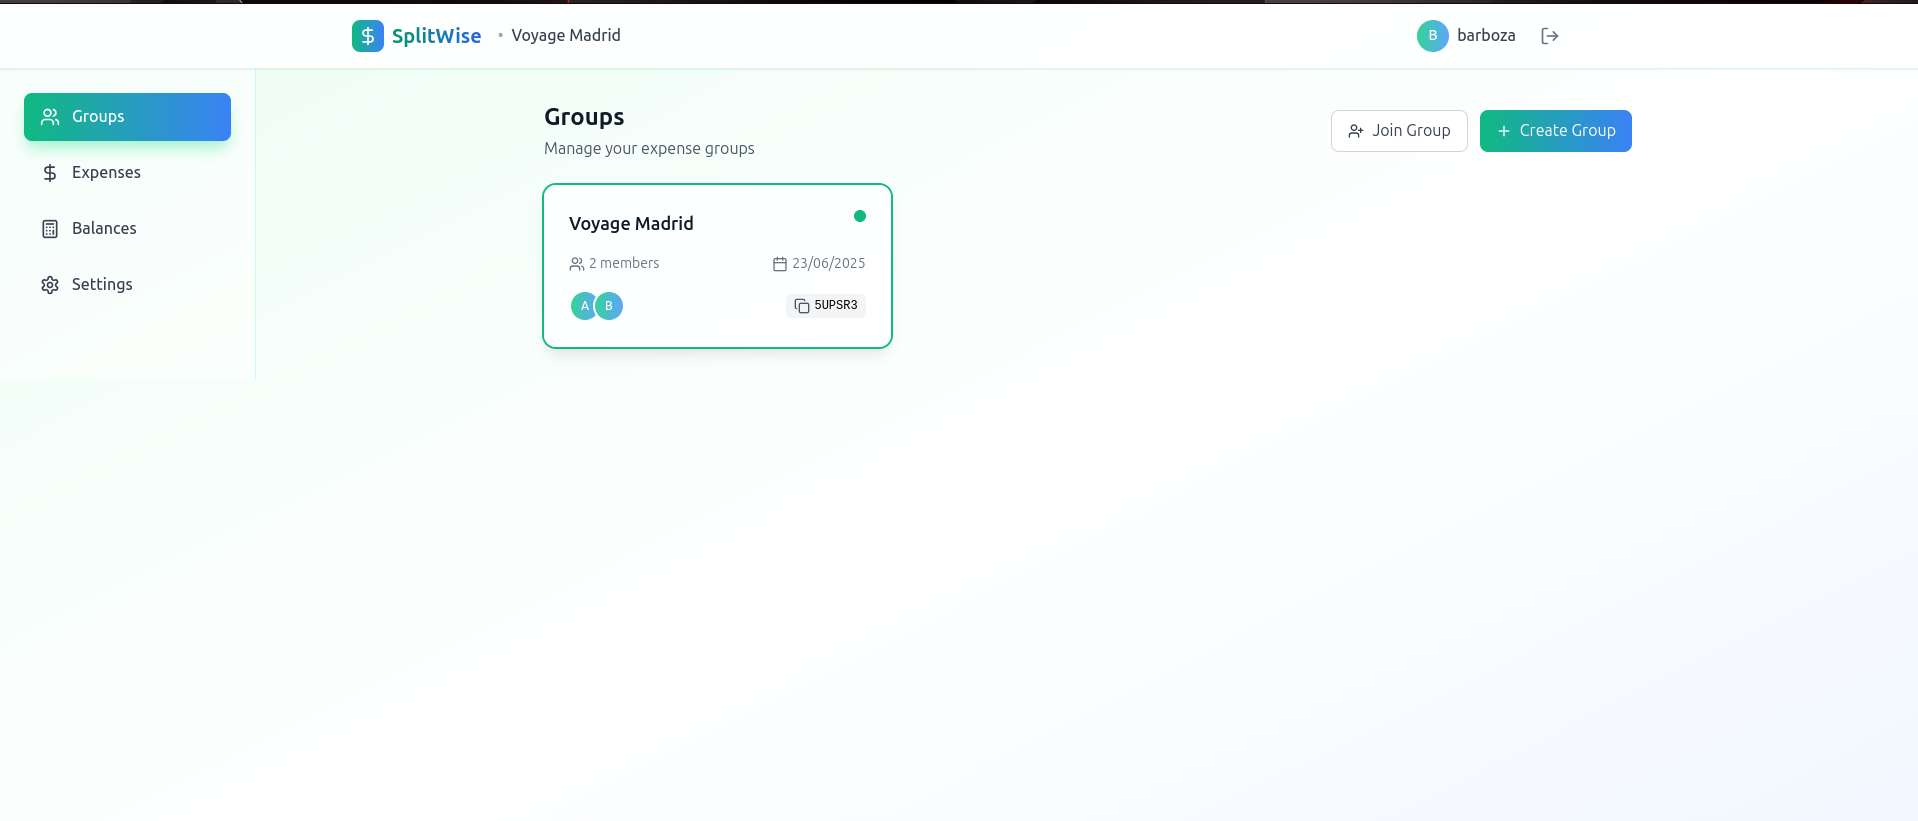
\includegraphics[width=0.2\textwidth]{app-screens/Groups_Screen.png}
\end{frame}

% Page 2 : Le prompt utilisé
\begin{frame}{Prompt utilisé pour générer l'application}
\textbf{Prompt donné à l'IA (ChatGPT/Bolt.new) :}
\begin{lstlisting}[language=,breaklines=true]
You are a professional react developper, build a responsive web applicatio that allows groups of users to easily manage and split shared expenses. The key features should include:

User Authentication:
Users can sign up, log in, and log out.
Optionally allow guest access without login.

Groups (or Trips):
Users can create groups (like a trip or event).
Users can invite others via email or share a link to join the group.
Each group has a unique page/dashboard.

Expense Management:
Users in the group can add expenses with fields:
Description, Amount, Date, Paid by, Shared by (equal or custom shares)
Edit and delete expenses.

Balances & Settlements:
Calculate how much each member owes or is owed.
Show a clear summary of who needs to pay whom and how much.
Optional: Suggest minimal transactions to settle all debts.

Notifications:
Notify users when expenses are added or updated.
Optionally notify when payments are settled.

User Interface:
Clean, intuitive, and mobile-friendly UI.
Show list of expenses, participants, and balances.
Use charts or graphs to visualize balances (optional).

Data Persistence:
Store data securely (using any backend  database).
Ensure data consistency when multiple users update at the same time.

Tech Stack Suggestion ():
Frontend: Vue.js
Backend: Node.js with Express
Database: MongoDB
\end{lstlisting}
\end{frame}

% Page 3 : Stack technique réelle
\begin{frame}{Stack technique réellement utilisée}
\begin{itemize}
  \item \textbf{Frontend :} React 18, TypeScript, Tailwind CSS, Vite
  \item \textbf{Gestion d'état :} Context API + useReducer
  \item \textbf{Persistance des données :} localStorage du navigateur
  \item \textbf{Backend :} Aucun (100\% front-end)
  \item \textbf{Base de données distante :} Aucune
\end{itemize}
\vspace{0.5em}
\textit{\small Toutes les données sont stockées localement dans le navigateur de l'utilisateur.}
\end{frame}

% Page 4 : Fonctionnement de l'application
\begin{frame}{Fonctionnement de l'application}
\begin{itemize}
  \item \textbf{Authentification :} Inscription, connexion, accès invité
  \item \textbf{Groupes :} Création, invitation, gestion des membres
  \item \textbf{Dépenses :} Ajout, édition, suppression, répartition flexible
  \item \textbf{Calculs :} Soldes automatiques, suggestions de remboursements
  \item \textbf{UI :} Moderne, responsive, mobile-friendly (voir captures)
  \item \textbf{Export/Import :} Sauvegarde/restauration des données en JSON
\end{itemize}
\begin{center}
  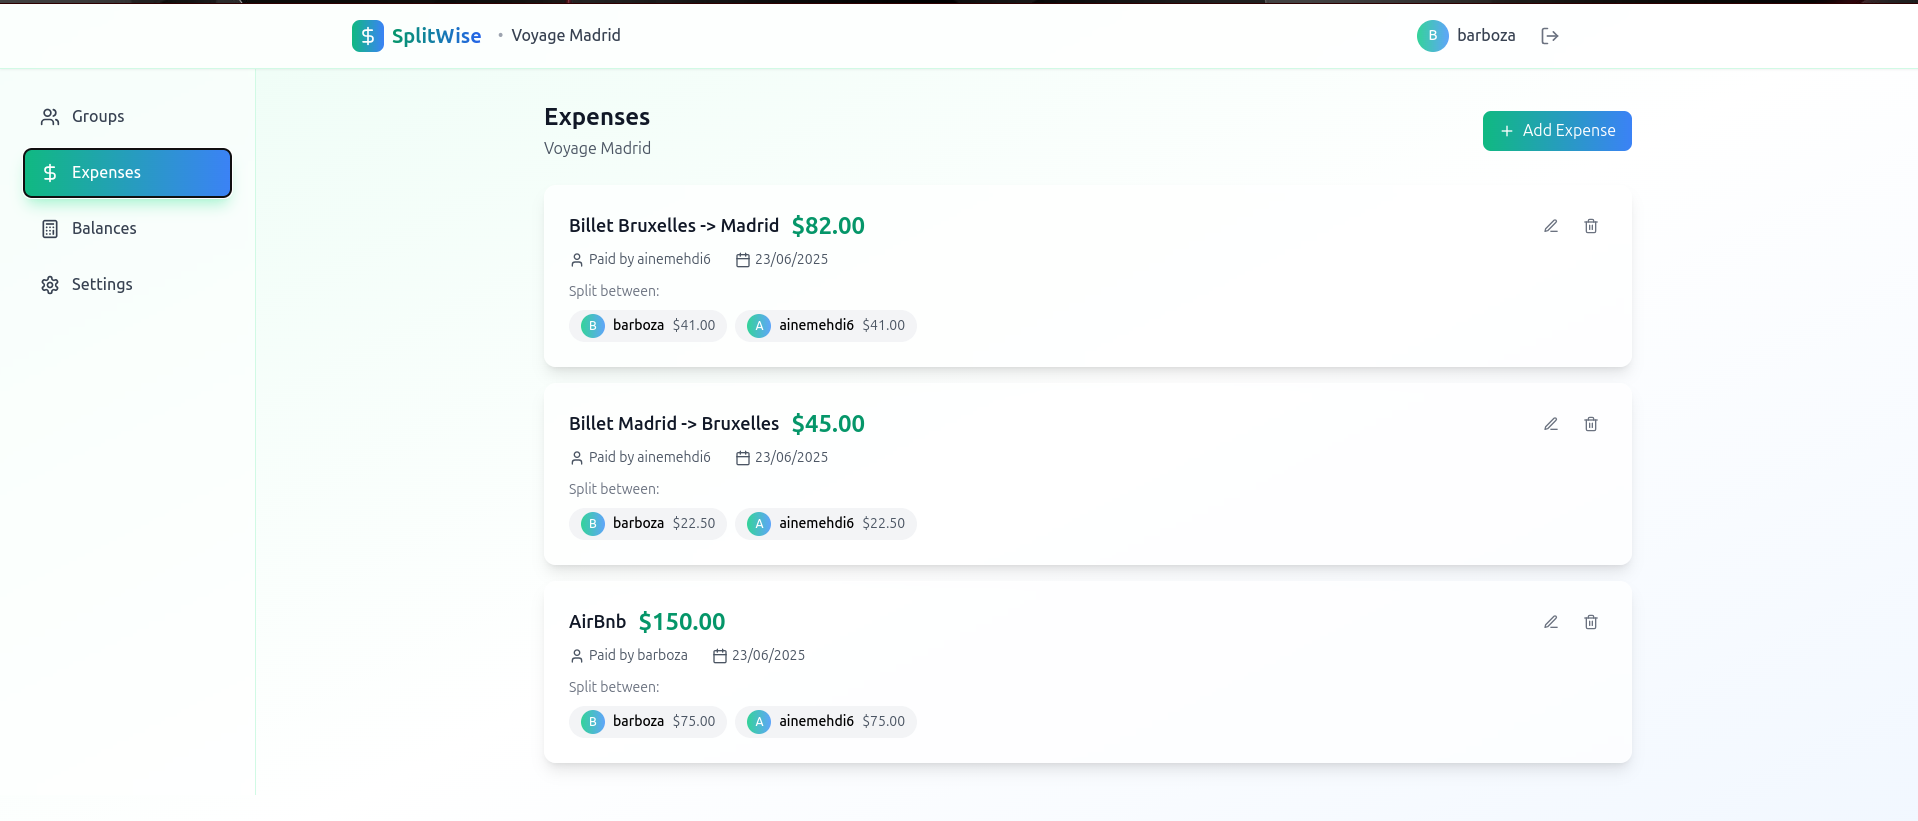
\includegraphics[width=0.35\textwidth]{app-screens/Expenses_Screen.png}
  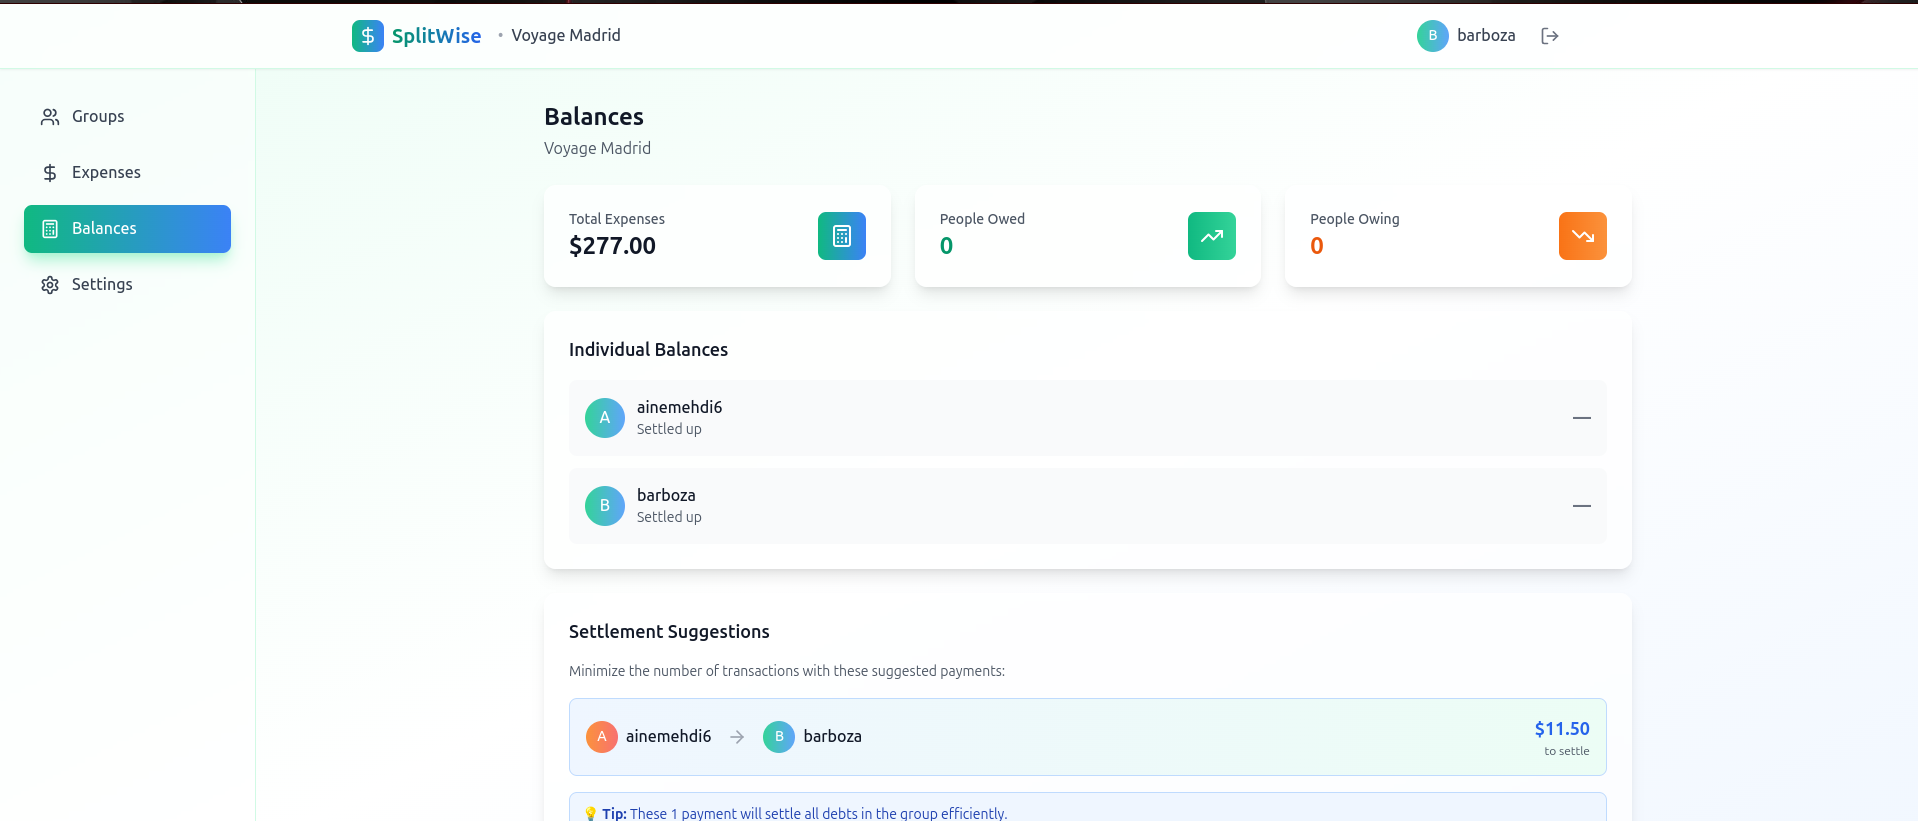
\includegraphics[width=0.35\textwidth]{app-screens/Balances_Screen.png}
\end{center}
\end{frame}

% Page 5 : Conclusion et démarche IA
\begin{frame}{Conclusion et démarche IA}
\begin{itemize}
  \item Utilisation de l'IA (ChatGPT, Bolt.new) pour générer la structure et les composants de l'application
  \item Amélioration et personnalisation du code avec Cursor
  \item Stack technique adaptée à un projet front-end moderne
  \item Application légère, rapide, sans backend ni base de données distante
\end{itemize}
\vspace{1em}
\textbf{Merci pour votre attention !}
\end{frame}

\end{document} 